% Created by tikzDevice version 0.12.6 on 2026-05-29 11:03:41
% !TEX encoding = UTF-8 Unicode
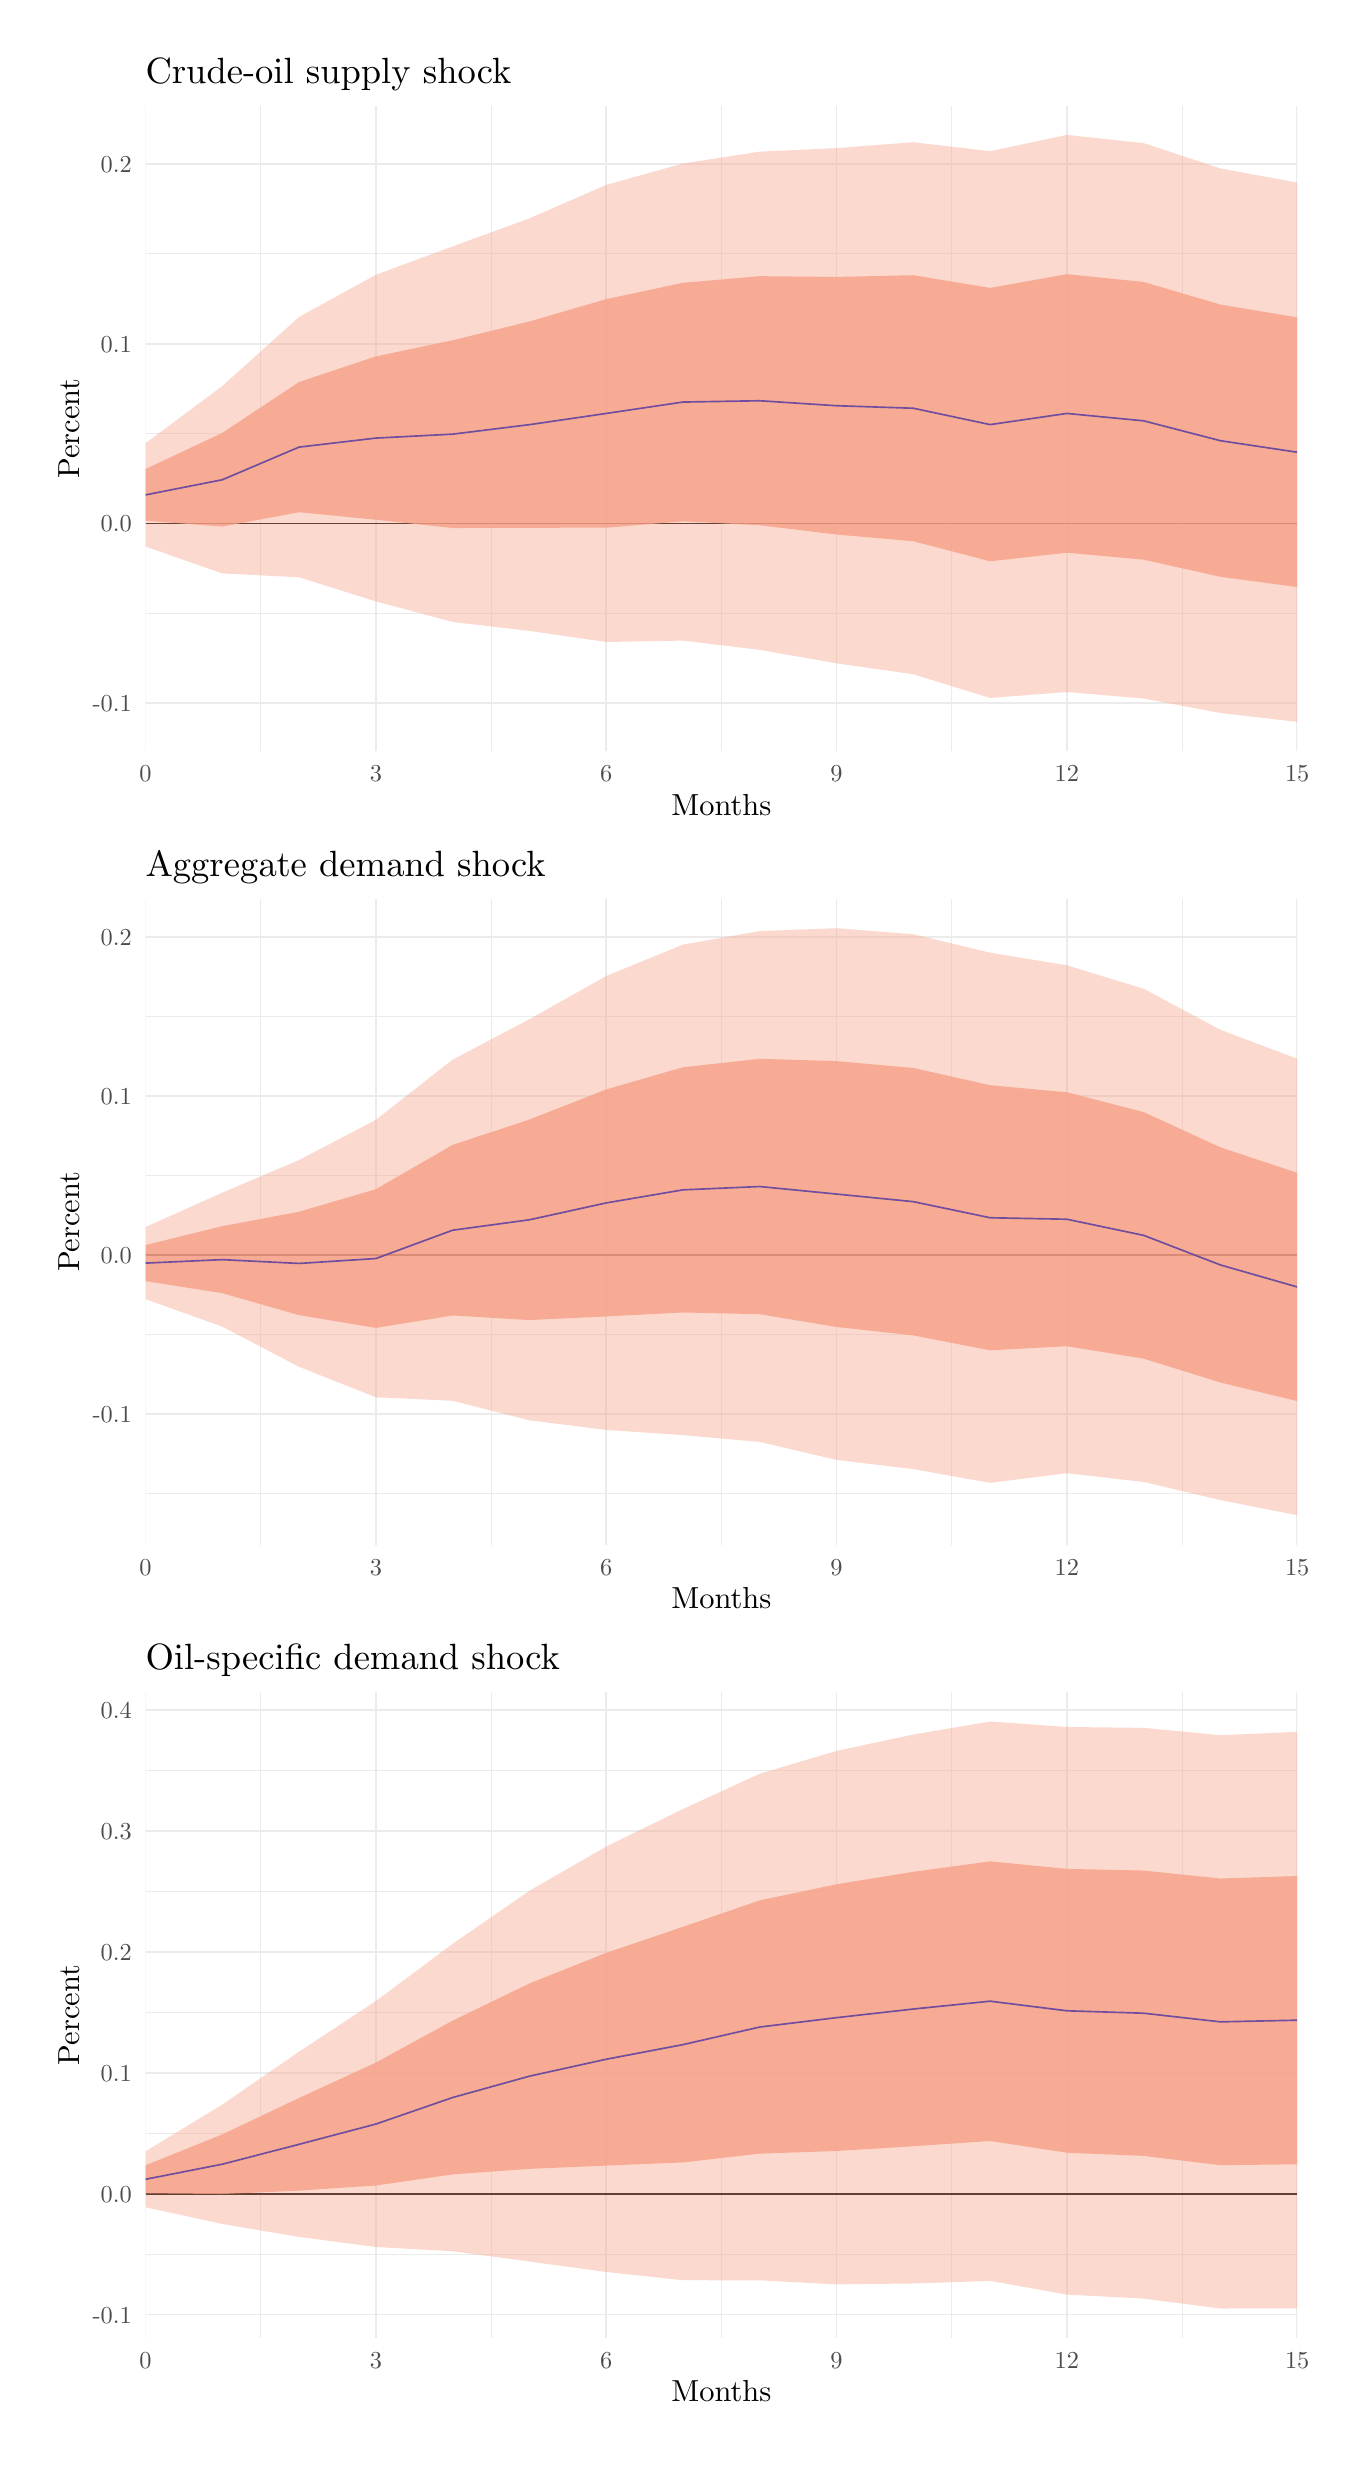
\begin{tikzpicture}[x=1pt,y=1pt]
\definecolor{fillColor}{RGB}{255,255,255}
\path[use as bounding box,fill=fillColor,fill opacity=0.00] (0,0) rectangle (469.75,870.97);
\begin{scope}
\path[clip] (  0.00,  0.00) rectangle (469.75,870.97);
\definecolor{fillColor}{RGB}{255,255,255}

\path[fill=fillColor] (  0.00,  0.00) rectangle (469.75,870.97);
\end{scope}
\begin{scope}
\path[clip] (  5.50,578.82) rectangle (464.25,865.47);
\definecolor{fillColor}{RGB}{255,255,255}

\path[fill=fillColor] (  5.50,578.82) rectangle (464.25,865.47);
\end{scope}
\begin{scope}
\path[clip] (  5.50,292.16) rectangle (464.25,578.82);
\definecolor{fillColor}{RGB}{255,255,255}

\path[fill=fillColor] (  5.50,292.16) rectangle (464.25,578.82);
\end{scope}
\begin{scope}
\path[clip] (  5.50,  5.50) rectangle (464.25,292.16);
\definecolor{fillColor}{RGB}{255,255,255}

\path[fill=fillColor] (  5.50,  5.50) rectangle (464.25,292.16);
\end{scope}
\begin{scope}
\path[clip] ( 42.59,609.50) rectangle (458.75,842.82);
\definecolor{drawColor}{gray}{0.92}

\path[draw=drawColor,line width= 0.3pt,line join=round] ( 42.59,659.30) --
	(458.75,659.30);

\path[draw=drawColor,line width= 0.3pt,line join=round] ( 42.59,724.28) --
	(458.75,724.28);

\path[draw=drawColor,line width= 0.3pt,line join=round] ( 42.59,789.25) --
	(458.75,789.25);

\path[draw=drawColor,line width= 0.3pt,line join=round] ( 84.21,609.50) --
	( 84.21,842.82);

\path[draw=drawColor,line width= 0.3pt,line join=round] (167.44,609.50) --
	(167.44,842.82);

\path[draw=drawColor,line width= 0.3pt,line join=round] (250.67,609.50) --
	(250.67,842.82);

\path[draw=drawColor,line width= 0.3pt,line join=round] (333.91,609.50) --
	(333.91,842.82);

\path[draw=drawColor,line width= 0.3pt,line join=round] (417.14,609.50) --
	(417.14,842.82);

\path[draw=drawColor,line width= 0.6pt,line join=round] ( 42.59,626.82) --
	(458.75,626.82);

\path[draw=drawColor,line width= 0.6pt,line join=round] ( 42.59,691.79) --
	(458.75,691.79);

\path[draw=drawColor,line width= 0.6pt,line join=round] ( 42.59,756.77) --
	(458.75,756.77);

\path[draw=drawColor,line width= 0.6pt,line join=round] ( 42.59,821.74) --
	(458.75,821.74);

\path[draw=drawColor,line width= 0.6pt,line join=round] ( 42.59,609.50) --
	( 42.59,842.82);

\path[draw=drawColor,line width= 0.6pt,line join=round] (125.82,609.50) --
	(125.82,842.82);

\path[draw=drawColor,line width= 0.6pt,line join=round] (209.06,609.50) --
	(209.06,842.82);

\path[draw=drawColor,line width= 0.6pt,line join=round] (292.29,609.50) --
	(292.29,842.82);

\path[draw=drawColor,line width= 0.6pt,line join=round] (375.52,609.50) --
	(375.52,842.82);

\path[draw=drawColor,line width= 0.6pt,line join=round] (458.75,609.50) --
	(458.75,842.82);
\definecolor{drawColor}{RGB}{0,0,0}

\path[draw=drawColor,line width= 0.6pt,line join=round] ( 42.59,691.79) -- (458.75,691.79);
\definecolor{fillColor}{RGB}{247,160,134}

\path[fill=fillColor,fill opacity=0.80] ( 42.59,711.46) --
	( 70.33,724.53) --
	( 98.08,742.92) --
	(125.82,752.16) --
	(153.57,758.00) --
	(181.31,764.78) --
	(209.06,772.85) --
	(236.80,778.77) --
	(264.54,781.16) --
	(292.29,780.89) --
	(320.03,781.51) --
	(347.78,776.92) --
	(375.52,781.89) --
	(403.27,779.06) --
	(431.01,770.90) --
	(458.75,766.27) --
	(458.75,668.83) --
	(431.01,672.53) --
	(403.27,678.72) --
	(375.52,681.24) --
	(347.78,678.14) --
	(320.03,685.38) --
	(292.29,687.81) --
	(264.54,691.15) --
	(236.80,692.58) --
	(209.06,690.27) --
	(181.31,690.25) --
	(153.57,690.15) --
	(125.82,693.16) --
	( 98.08,695.87) --
	( 70.33,690.68) --
	( 42.59,692.80) --
	cycle;

\path[] ( 42.59,711.46) --
	( 70.33,724.53) --
	( 98.08,742.92) --
	(125.82,752.16) --
	(153.57,758.00) --
	(181.31,764.78) --
	(209.06,772.85) --
	(236.80,778.77) --
	(264.54,781.16) --
	(292.29,780.89) --
	(320.03,781.51) --
	(347.78,776.92) --
	(375.52,781.89) --
	(403.27,779.06) --
	(431.01,770.90) --
	(458.75,766.27);

\path[] (458.75,668.83) --
	(431.01,672.53) --
	(403.27,678.72) --
	(375.52,681.24) --
	(347.78,678.14) --
	(320.03,685.38) --
	(292.29,687.81) --
	(264.54,691.15) --
	(236.80,692.58) --
	(209.06,690.27) --
	(181.31,690.25) --
	(153.57,690.15) --
	(125.82,693.16) --
	( 98.08,695.87) --
	( 70.33,690.68) --
	( 42.59,692.80);
\definecolor{fillColor}{RGB}{247,160,134}

\path[fill=fillColor,fill opacity=0.40] ( 42.59,720.80) --
	( 70.33,741.45) --
	( 98.08,766.45) --
	(125.82,781.66) --
	(153.57,791.93) --
	(181.31,802.04) --
	(209.06,814.14) --
	(236.80,821.87) --
	(264.54,826.17) --
	(292.29,827.44) --
	(320.03,829.57) --
	(347.78,826.31) --
	(375.52,832.21) --
	(403.27,829.23) --
	(431.01,820.08) --
	(458.75,814.99) --
	(458.75,620.11) --
	(431.01,623.34) --
	(403.27,628.55) --
	(375.52,630.91) --
	(347.78,628.75) --
	(320.03,637.32) --
	(292.29,641.26) --
	(264.54,646.14) --
	(236.80,649.48) --
	(209.06,648.98) --
	(181.31,652.98) --
	(153.57,656.22) --
	(125.82,663.66) --
	( 98.08,672.35) --
	( 70.33,673.75) --
	( 42.59,683.47) --
	cycle;

\path[] ( 42.59,720.80) --
	( 70.33,741.45) --
	( 98.08,766.45) --
	(125.82,781.66) --
	(153.57,791.93) --
	(181.31,802.04) --
	(209.06,814.14) --
	(236.80,821.87) --
	(264.54,826.17) --
	(292.29,827.44) --
	(320.03,829.57) --
	(347.78,826.31) --
	(375.52,832.21) --
	(403.27,829.23) --
	(431.01,820.08) --
	(458.75,814.99);

\path[] (458.75,620.11) --
	(431.01,623.34) --
	(403.27,628.55) --
	(375.52,630.91) --
	(347.78,628.75) --
	(320.03,637.32) --
	(292.29,641.26) --
	(264.54,646.14) --
	(236.80,649.48) --
	(209.06,648.98) --
	(181.31,652.98) --
	(153.57,656.22) --
	(125.82,663.66) --
	( 98.08,672.35) --
	( 70.33,673.75) --
	( 42.59,683.47);
\definecolor{drawColor}{RGB}{112,77,158}

\path[draw=drawColor,line width= 0.6pt,line join=round] ( 42.59,702.13) --
	( 70.33,707.60) --
	( 98.08,719.40) --
	(125.82,722.66) --
	(153.57,724.08) --
	(181.31,727.51) --
	(209.06,731.56) --
	(236.80,735.68) --
	(264.54,736.15) --
	(292.29,734.35) --
	(320.03,733.44) --
	(347.78,727.53) --
	(375.52,731.56) --
	(403.27,728.89) --
	(431.01,721.71) --
	(458.75,717.55);
\end{scope}
\begin{scope}
\path[clip] (  0.00,  0.00) rectangle (469.75,870.97);
\definecolor{drawColor}{gray}{0.30}

\node[text=drawColor,anchor=base east,inner sep=0pt, outer sep=0pt, scale=  0.88] at ( 37.64,623.79) {-0.1};

\node[text=drawColor,anchor=base east,inner sep=0pt, outer sep=0pt, scale=  0.88] at ( 37.64,688.76) {0.0};

\node[text=drawColor,anchor=base east,inner sep=0pt, outer sep=0pt, scale=  0.88] at ( 37.64,753.74) {0.1};

\node[text=drawColor,anchor=base east,inner sep=0pt, outer sep=0pt, scale=  0.88] at ( 37.64,818.71) {0.2};
\end{scope}
\begin{scope}
\path[clip] (  0.00,  0.00) rectangle (469.75,870.97);
\definecolor{drawColor}{gray}{0.30}

\node[text=drawColor,anchor=base,inner sep=0pt, outer sep=0pt, scale=  0.88] at ( 42.59,598.49) {0};

\node[text=drawColor,anchor=base,inner sep=0pt, outer sep=0pt, scale=  0.88] at (125.82,598.49) {3};

\node[text=drawColor,anchor=base,inner sep=0pt, outer sep=0pt, scale=  0.88] at (209.06,598.49) {6};

\node[text=drawColor,anchor=base,inner sep=0pt, outer sep=0pt, scale=  0.88] at (292.29,598.49) {9};

\node[text=drawColor,anchor=base,inner sep=0pt, outer sep=0pt, scale=  0.88] at (375.52,598.49) {12};

\node[text=drawColor,anchor=base,inner sep=0pt, outer sep=0pt, scale=  0.88] at (458.75,598.49) {15};
\end{scope}
\begin{scope}
\path[clip] (  0.00,  0.00) rectangle (469.75,870.97);
\definecolor{drawColor}{RGB}{0,0,0}

\node[text=drawColor,anchor=base,inner sep=0pt, outer sep=0pt, scale=  1.10] at (250.67,586.45) {Months};
\end{scope}
\begin{scope}
\path[clip] (  0.00,  0.00) rectangle (469.75,870.97);
\definecolor{drawColor}{RGB}{0,0,0}

\node[text=drawColor,rotate= 90.00,anchor=base,inner sep=0pt, outer sep=0pt, scale=  1.10] at ( 18.58,726.16) {Percent};
\end{scope}
\begin{scope}
\path[clip] (  0.00,  0.00) rectangle (469.75,870.97);
\definecolor{drawColor}{RGB}{0,0,0}

\node[text=drawColor,anchor=base west,inner sep=0pt, outer sep=0pt, scale=  1.32] at ( 42.59,850.88) {Crude-oil supply shock};
\end{scope}
\begin{scope}
\path[clip] ( 42.59,322.84) rectangle (458.75,556.16);
\definecolor{drawColor}{gray}{0.92}

\path[draw=drawColor,line width= 0.3pt,line join=round] ( 42.59,341.41) --
	(458.75,341.41);

\path[draw=drawColor,line width= 0.3pt,line join=round] ( 42.59,398.83) --
	(458.75,398.83);

\path[draw=drawColor,line width= 0.3pt,line join=round] ( 42.59,456.24) --
	(458.75,456.24);

\path[draw=drawColor,line width= 0.3pt,line join=round] ( 42.59,513.65) --
	(458.75,513.65);

\path[draw=drawColor,line width= 0.3pt,line join=round] ( 84.21,322.84) --
	( 84.21,556.16);

\path[draw=drawColor,line width= 0.3pt,line join=round] (167.44,322.84) --
	(167.44,556.16);

\path[draw=drawColor,line width= 0.3pt,line join=round] (250.67,322.84) --
	(250.67,556.16);

\path[draw=drawColor,line width= 0.3pt,line join=round] (333.91,322.84) --
	(333.91,556.16);

\path[draw=drawColor,line width= 0.3pt,line join=round] (417.14,322.84) --
	(417.14,556.16);

\path[draw=drawColor,line width= 0.6pt,line join=round] ( 42.59,370.12) --
	(458.75,370.12);

\path[draw=drawColor,line width= 0.6pt,line join=round] ( 42.59,427.53) --
	(458.75,427.53);

\path[draw=drawColor,line width= 0.6pt,line join=round] ( 42.59,484.94) --
	(458.75,484.94);

\path[draw=drawColor,line width= 0.6pt,line join=round] ( 42.59,542.35) --
	(458.75,542.35);

\path[draw=drawColor,line width= 0.6pt,line join=round] ( 42.59,322.84) --
	( 42.59,556.16);

\path[draw=drawColor,line width= 0.6pt,line join=round] (125.82,322.84) --
	(125.82,556.16);

\path[draw=drawColor,line width= 0.6pt,line join=round] (209.06,322.84) --
	(209.06,556.16);

\path[draw=drawColor,line width= 0.6pt,line join=round] (292.29,322.84) --
	(292.29,556.16);

\path[draw=drawColor,line width= 0.6pt,line join=round] (375.52,322.84) --
	(375.52,556.16);

\path[draw=drawColor,line width= 0.6pt,line join=round] (458.75,322.84) --
	(458.75,556.16);
\definecolor{drawColor}{RGB}{0,0,0}

\path[draw=drawColor,line width= 0.6pt,line join=round] ( 42.59,427.53) -- (458.75,427.53);
\definecolor{fillColor}{RGB}{247,160,134}

\path[fill=fillColor,fill opacity=0.80] ( 42.59,431.05) --
	( 70.33,437.89) --
	( 98.08,443.10) --
	(125.82,451.25) --
	(153.57,467.24) --
	(181.31,476.42) --
	(209.06,487.29) --
	(236.80,495.31) --
	(264.54,498.36) --
	(292.29,497.52) --
	(320.03,495.05) --
	(347.78,488.82) --
	(375.52,486.27) --
	(403.27,479.11) --
	(431.01,466.35) --
	(458.75,457.15) --
	(458.75,374.68) --
	(431.01,381.39) --
	(403.27,390.01) --
	(375.52,394.51) --
	(347.78,393.03) --
	(320.03,398.42) --
	(292.29,401.46) --
	(264.54,406.06) --
	(236.80,406.70) --
	(209.06,405.28) --
	(181.31,403.96) --
	(153.57,405.61) --
	(125.82,401.13) --
	( 98.08,405.74) --
	( 70.33,413.68) --
	( 42.59,418.03) --
	cycle;

\path[] ( 42.59,431.05) --
	( 70.33,437.89) --
	( 98.08,443.10) --
	(125.82,451.25) --
	(153.57,467.24) --
	(181.31,476.42) --
	(209.06,487.29) --
	(236.80,495.31) --
	(264.54,498.36) --
	(292.29,497.52) --
	(320.03,495.05) --
	(347.78,488.82) --
	(375.52,486.27) --
	(403.27,479.11) --
	(431.01,466.35) --
	(458.75,457.15);

\path[] (458.75,374.68) --
	(431.01,381.39) --
	(403.27,390.01) --
	(375.52,394.51) --
	(347.78,393.03) --
	(320.03,398.42) --
	(292.29,401.46) --
	(264.54,406.06) --
	(236.80,406.70) --
	(209.06,405.28) --
	(181.31,403.96) --
	(153.57,405.61) --
	(125.82,401.13) --
	( 98.08,405.74) --
	( 70.33,413.68) --
	( 42.59,418.03);
\definecolor{fillColor}{RGB}{247,160,134}

\path[fill=fillColor,fill opacity=0.40] ( 42.59,437.57) --
	( 70.33,449.99) --
	( 98.08,461.78) --
	(125.82,476.31) --
	(153.57,498.06) --
	(181.31,512.66) --
	(209.06,528.30) --
	(236.80,539.62) --
	(264.54,544.51) --
	(292.29,545.55) --
	(320.03,543.37) --
	(347.78,536.71) --
	(375.52,532.15) --
	(403.27,523.66) --
	(431.01,508.83) --
	(458.75,498.38) --
	(458.75,333.45) --
	(431.01,338.91) --
	(403.27,345.46) --
	(375.52,348.63) --
	(347.78,345.14) --
	(320.03,350.10) --
	(292.29,353.43) --
	(264.54,359.92) --
	(236.80,362.39) --
	(209.06,364.27) --
	(181.31,367.73) --
	(153.57,374.79) --
	(125.82,376.07) --
	( 98.08,387.06) --
	( 70.33,401.58) --
	( 42.59,411.52) --
	cycle;

\path[] ( 42.59,437.57) --
	( 70.33,449.99) --
	( 98.08,461.78) --
	(125.82,476.31) --
	(153.57,498.06) --
	(181.31,512.66) --
	(209.06,528.30) --
	(236.80,539.62) --
	(264.54,544.51) --
	(292.29,545.55) --
	(320.03,543.37) --
	(347.78,536.71) --
	(375.52,532.15) --
	(403.27,523.66) --
	(431.01,508.83) --
	(458.75,498.38);

\path[] (458.75,333.45) --
	(431.01,338.91) --
	(403.27,345.46) --
	(375.52,348.63) --
	(347.78,345.14) --
	(320.03,350.10) --
	(292.29,353.43) --
	(264.54,359.92) --
	(236.80,362.39) --
	(209.06,364.27) --
	(181.31,367.73) --
	(153.57,374.79) --
	(125.82,376.07) --
	( 98.08,387.06) --
	( 70.33,401.58) --
	( 42.59,411.52);
\definecolor{drawColor}{RGB}{112,77,158}

\path[draw=drawColor,line width= 0.6pt,line join=round] ( 42.59,424.54) --
	( 70.33,425.79) --
	( 98.08,424.42) --
	(125.82,426.19) --
	(153.57,436.43) --
	(181.31,440.19) --
	(209.06,446.29) --
	(236.80,451.01) --
	(264.54,452.21) --
	(292.29,449.49) --
	(320.03,446.74) --
	(347.78,440.93) --
	(375.52,440.39) --
	(403.27,434.56) --
	(431.01,423.87) --
	(458.75,415.92);
\end{scope}
\begin{scope}
\path[clip] (  0.00,  0.00) rectangle (469.75,870.97);
\definecolor{drawColor}{gray}{0.30}

\node[text=drawColor,anchor=base east,inner sep=0pt, outer sep=0pt, scale=  0.88] at ( 37.64,367.09) {-0.1};

\node[text=drawColor,anchor=base east,inner sep=0pt, outer sep=0pt, scale=  0.88] at ( 37.64,424.50) {0.0};

\node[text=drawColor,anchor=base east,inner sep=0pt, outer sep=0pt, scale=  0.88] at ( 37.64,481.91) {0.1};

\node[text=drawColor,anchor=base east,inner sep=0pt, outer sep=0pt, scale=  0.88] at ( 37.64,539.32) {0.2};
\end{scope}
\begin{scope}
\path[clip] (  0.00,  0.00) rectangle (469.75,870.97);
\definecolor{drawColor}{gray}{0.30}

\node[text=drawColor,anchor=base,inner sep=0pt, outer sep=0pt, scale=  0.88] at ( 42.59,311.83) {0};

\node[text=drawColor,anchor=base,inner sep=0pt, outer sep=0pt, scale=  0.88] at (125.82,311.83) {3};

\node[text=drawColor,anchor=base,inner sep=0pt, outer sep=0pt, scale=  0.88] at (209.06,311.83) {6};

\node[text=drawColor,anchor=base,inner sep=0pt, outer sep=0pt, scale=  0.88] at (292.29,311.83) {9};

\node[text=drawColor,anchor=base,inner sep=0pt, outer sep=0pt, scale=  0.88] at (375.52,311.83) {12};

\node[text=drawColor,anchor=base,inner sep=0pt, outer sep=0pt, scale=  0.88] at (458.75,311.83) {15};
\end{scope}
\begin{scope}
\path[clip] (  0.00,  0.00) rectangle (469.75,870.97);
\definecolor{drawColor}{RGB}{0,0,0}

\node[text=drawColor,anchor=base,inner sep=0pt, outer sep=0pt, scale=  1.10] at (250.67,299.80) {Months};
\end{scope}
\begin{scope}
\path[clip] (  0.00,  0.00) rectangle (469.75,870.97);
\definecolor{drawColor}{RGB}{0,0,0}

\node[text=drawColor,rotate= 90.00,anchor=base,inner sep=0pt, outer sep=0pt, scale=  1.10] at ( 18.58,439.50) {Percent};
\end{scope}
\begin{scope}
\path[clip] (  0.00,  0.00) rectangle (469.75,870.97);
\definecolor{drawColor}{RGB}{0,0,0}

\node[text=drawColor,anchor=base west,inner sep=0pt, outer sep=0pt, scale=  1.32] at ( 42.59,564.22) {Aggregate demand shock};
\end{scope}
\begin{scope}
\path[clip] ( 42.59, 36.19) rectangle (458.75,269.50);
\definecolor{drawColor}{gray}{0.92}

\path[draw=drawColor,line width= 0.3pt,line join=round] ( 42.59, 66.43) --
	(458.75, 66.43);

\path[draw=drawColor,line width= 0.3pt,line join=round] ( 42.59,110.13) --
	(458.75,110.13);

\path[draw=drawColor,line width= 0.3pt,line join=round] ( 42.59,153.83) --
	(458.75,153.83);

\path[draw=drawColor,line width= 0.3pt,line join=round] ( 42.59,197.53) --
	(458.75,197.53);

\path[draw=drawColor,line width= 0.3pt,line join=round] ( 42.59,241.22) --
	(458.75,241.22);

\path[draw=drawColor,line width= 0.3pt,line join=round] ( 84.21, 36.19) --
	( 84.21,269.50);

\path[draw=drawColor,line width= 0.3pt,line join=round] (167.44, 36.19) --
	(167.44,269.50);

\path[draw=drawColor,line width= 0.3pt,line join=round] (250.67, 36.19) --
	(250.67,269.50);

\path[draw=drawColor,line width= 0.3pt,line join=round] (333.91, 36.19) --
	(333.91,269.50);

\path[draw=drawColor,line width= 0.3pt,line join=round] (417.14, 36.19) --
	(417.14,269.50);

\path[draw=drawColor,line width= 0.6pt,line join=round] ( 42.59, 44.58) --
	(458.75, 44.58);

\path[draw=drawColor,line width= 0.6pt,line join=round] ( 42.59, 88.28) --
	(458.75, 88.28);

\path[draw=drawColor,line width= 0.6pt,line join=round] ( 42.59,131.98) --
	(458.75,131.98);

\path[draw=drawColor,line width= 0.6pt,line join=round] ( 42.59,175.68) --
	(458.75,175.68);

\path[draw=drawColor,line width= 0.6pt,line join=round] ( 42.59,219.37) --
	(458.75,219.37);

\path[draw=drawColor,line width= 0.6pt,line join=round] ( 42.59,263.07) --
	(458.75,263.07);

\path[draw=drawColor,line width= 0.6pt,line join=round] ( 42.59, 36.19) --
	( 42.59,269.50);

\path[draw=drawColor,line width= 0.6pt,line join=round] (125.82, 36.19) --
	(125.82,269.50);

\path[draw=drawColor,line width= 0.6pt,line join=round] (209.06, 36.19) --
	(209.06,269.50);

\path[draw=drawColor,line width= 0.6pt,line join=round] (292.29, 36.19) --
	(292.29,269.50);

\path[draw=drawColor,line width= 0.6pt,line join=round] (375.52, 36.19) --
	(375.52,269.50);

\path[draw=drawColor,line width= 0.6pt,line join=round] (458.75, 36.19) --
	(458.75,269.50);
\definecolor{drawColor}{RGB}{0,0,0}

\path[draw=drawColor,line width= 0.6pt,line join=round] ( 42.59, 88.28) -- (458.75, 88.28);
\definecolor{fillColor}{RGB}{247,160,134}

\path[fill=fillColor,fill opacity=0.80] ( 42.59, 98.53) --
	( 70.33,109.71) --
	( 98.08,122.86) --
	(125.82,135.65) --
	(153.57,150.80) --
	(181.31,164.24) --
	(209.06,175.29) --
	(236.80,184.71) --
	(264.54,194.26) --
	(292.29,200.08) --
	(320.03,204.59) --
	(347.78,208.37) --
	(375.52,205.65) --
	(403.27,205.04) --
	(431.01,202.16) --
	(458.75,203.06) --
	(458.75, 98.89) --
	(431.01, 98.58) --
	(403.27,101.93) --
	(375.52,103.09) --
	(347.78,107.32) --
	(320.03,105.42) --
	(292.29,103.71) --
	(264.54,102.74) --
	(236.80, 99.58) --
	(209.06, 98.43) --
	(181.31, 97.25) --
	(153.57, 95.26) --
	(125.82, 91.23) --
	( 98.08, 89.38) --
	( 70.33, 88.15) --
	( 42.59, 88.43) --
	cycle;

\path[] ( 42.59, 98.53) --
	( 70.33,109.71) --
	( 98.08,122.86) --
	(125.82,135.65) --
	(153.57,150.80) --
	(181.31,164.24) --
	(209.06,175.29) --
	(236.80,184.71) --
	(264.54,194.26) --
	(292.29,200.08) --
	(320.03,204.59) --
	(347.78,208.37) --
	(375.52,205.65) --
	(403.27,205.04) --
	(431.01,202.16) --
	(458.75,203.06);

\path[] (458.75, 98.89) --
	(431.01, 98.58) --
	(403.27,101.93) --
	(375.52,103.09) --
	(347.78,107.32) --
	(320.03,105.42) --
	(292.29,103.71) --
	(264.54,102.74) --
	(236.80, 99.58) --
	(209.06, 98.43) --
	(181.31, 97.25) --
	(153.57, 95.26) --
	(125.82, 91.23) --
	( 98.08, 89.38) --
	( 70.33, 88.15) --
	( 42.59, 88.43);
\definecolor{fillColor}{RGB}{247,160,134}

\path[fill=fillColor,fill opacity=0.40] ( 42.59,103.58) --
	( 70.33,120.49) --
	( 98.08,139.60) --
	(125.82,157.86) --
	(153.57,178.57) --
	(181.31,197.73) --
	(209.06,213.72) --
	(236.80,227.28) --
	(264.54,240.02) --
	(292.29,248.27) --
	(320.03,254.18) --
	(347.78,258.90) --
	(375.52,256.92) --
	(403.27,256.60) --
	(431.01,253.94) --
	(458.75,255.14) --
	(458.75, 46.81) --
	(431.01, 46.79) --
	(403.27, 50.38) --
	(375.52, 51.82) --
	(347.78, 56.79) --
	(320.03, 55.83) --
	(292.29, 55.52) --
	(264.54, 56.98) --
	(236.80, 57.01) --
	(209.06, 59.99) --
	(181.31, 63.76) --
	(153.57, 67.49) --
	(125.82, 69.02) --
	( 98.08, 72.64) --
	( 70.33, 77.36) --
	( 42.59, 83.38) --
	cycle;

\path[] ( 42.59,103.58) --
	( 70.33,120.49) --
	( 98.08,139.60) --
	(125.82,157.86) --
	(153.57,178.57) --
	(181.31,197.73) --
	(209.06,213.72) --
	(236.80,227.28) --
	(264.54,240.02) --
	(292.29,248.27) --
	(320.03,254.18) --
	(347.78,258.90) --
	(375.52,256.92) --
	(403.27,256.60) --
	(431.01,253.94) --
	(458.75,255.14);

\path[] (458.75, 46.81) --
	(431.01, 46.79) --
	(403.27, 50.38) --
	(375.52, 51.82) --
	(347.78, 56.79) --
	(320.03, 55.83) --
	(292.29, 55.52) --
	(264.54, 56.98) --
	(236.80, 57.01) --
	(209.06, 59.99) --
	(181.31, 63.76) --
	(153.57, 67.49) --
	(125.82, 69.02) --
	( 98.08, 72.64) --
	( 70.33, 77.36) --
	( 42.59, 83.38);
\definecolor{drawColor}{RGB}{112,77,158}

\path[draw=drawColor,line width= 0.6pt,line join=round] ( 42.59, 93.48) --
	( 70.33, 98.93) --
	( 98.08,106.12) --
	(125.82,113.44) --
	(153.57,123.03) --
	(181.31,130.74) --
	(209.06,136.86) --
	(236.80,142.14) --
	(264.54,148.50) --
	(292.29,151.89) --
	(320.03,155.00) --
	(347.78,157.84) --
	(375.52,154.37) --
	(403.27,153.49) --
	(431.01,150.37) --
	(458.75,150.97);
\end{scope}
\begin{scope}
\path[clip] (  0.00,  0.00) rectangle (469.75,870.97);
\definecolor{drawColor}{gray}{0.30}

\node[text=drawColor,anchor=base east,inner sep=0pt, outer sep=0pt, scale=  0.88] at ( 37.64, 41.55) {-0.1};

\node[text=drawColor,anchor=base east,inner sep=0pt, outer sep=0pt, scale=  0.88] at ( 37.64, 85.25) {0.0};

\node[text=drawColor,anchor=base east,inner sep=0pt, outer sep=0pt, scale=  0.88] at ( 37.64,128.95) {0.1};

\node[text=drawColor,anchor=base east,inner sep=0pt, outer sep=0pt, scale=  0.88] at ( 37.64,172.64) {0.2};

\node[text=drawColor,anchor=base east,inner sep=0pt, outer sep=0pt, scale=  0.88] at ( 37.64,216.34) {0.3};

\node[text=drawColor,anchor=base east,inner sep=0pt, outer sep=0pt, scale=  0.88] at ( 37.64,260.04) {0.4};
\end{scope}
\begin{scope}
\path[clip] (  0.00,  0.00) rectangle (469.75,870.97);
\definecolor{drawColor}{gray}{0.30}

\node[text=drawColor,anchor=base,inner sep=0pt, outer sep=0pt, scale=  0.88] at ( 42.59, 25.18) {0};

\node[text=drawColor,anchor=base,inner sep=0pt, outer sep=0pt, scale=  0.88] at (125.82, 25.18) {3};

\node[text=drawColor,anchor=base,inner sep=0pt, outer sep=0pt, scale=  0.88] at (209.06, 25.18) {6};

\node[text=drawColor,anchor=base,inner sep=0pt, outer sep=0pt, scale=  0.88] at (292.29, 25.18) {9};

\node[text=drawColor,anchor=base,inner sep=0pt, outer sep=0pt, scale=  0.88] at (375.52, 25.18) {12};

\node[text=drawColor,anchor=base,inner sep=0pt, outer sep=0pt, scale=  0.88] at (458.75, 25.18) {15};
\end{scope}
\begin{scope}
\path[clip] (  0.00,  0.00) rectangle (469.75,870.97);
\definecolor{drawColor}{RGB}{0,0,0}

\node[text=drawColor,anchor=base,inner sep=0pt, outer sep=0pt, scale=  1.10] at (250.67, 13.14) {Months};
\end{scope}
\begin{scope}
\path[clip] (  0.00,  0.00) rectangle (469.75,870.97);
\definecolor{drawColor}{RGB}{0,0,0}

\node[text=drawColor,rotate= 90.00,anchor=base,inner sep=0pt, outer sep=0pt, scale=  1.10] at ( 18.58,152.84) {Percent};
\end{scope}
\begin{scope}
\path[clip] (  0.00,  0.00) rectangle (469.75,870.97);
\definecolor{drawColor}{RGB}{0,0,0}

\node[text=drawColor,anchor=base west,inner sep=0pt, outer sep=0pt, scale=  1.32] at ( 42.59,277.57) {Oil-specific demand shock};
\end{scope}
\end{tikzpicture}
